%%%%%%%%%%%%%%%%%%%%%%%%%%%%%%%%%%%%%%%%%%%%%%%%%%%%%%%%%%%%%%%%%
\chapter{BLOCK CIPHERS}\label{blockCiphers}
%%%%%%%%%%%%%%%%%%%%%%%%%%%%%%%%%%%%%%%%%%%%%%%%%%%%%%%%%%%%%%%%%
Block ciphers are main elements in symmetric cryptography, designed to securely encrypt message with symmetric key to obtain ciphertext. Block ciphers ensures data confidentiality. This chapter explores four primary structures of block ciphers: Substitution-Permutation Network (SPN), Feistel Network, ARX and Sponge construction. Each structure has distinct characteristics and design principles that contribute to their efficiency in cryptographic applications. 
\section{SPN}

The Substitution-Permutation Network (SPN) is a highly effective and widely adopted structure in block cipher design. SPN ciphers achieve encryption through a series of substitution and permutation operations applied over multiple rounds. This design ensures both confusion and diffusion, two fundamental principles in cryptographic security. An SPN cipher typically involves the following components:

\subsection{Substitution Boxes (S-Boxes)}
S-boxes are non-linear transformation tables that replace bits or bytes based on predefined mapping. The non-linearity of S-boxes is crucial for providing confusion, making it difficult for attackers to find relationships between key and ciphertext.

\subsection{Permutation Layer}
This layer permutes or shuffles the bits or bytes based on predifined mapping to ensure propagating the input-bit effect through the cipher structure to achieve uniform diffusion. 

\newpage
\subsection{Key Addition}
In each round, round key derived from the master key with some key-schedule is XORed with the current round's ciphertext. Key addition makes encryption process depend into subkeys derived from master key, ensuring that different keys produce different ciphertexts even for the same plaintext. Basic structure of SPN is shown in Figure \ref{fig:SPN} 


\subsection{The design principle of SPN}
The design of SPN ciphers is guided by several key principles to ensure high levels of security:

    \begin{itemize}
        \item Non-linearity is achieved through S-boxes, non-linearity is crucial to preventing linear relationships between the plaintext and ciphertext.
        \item  The permutation layer ensures that the influence of each input bit is spread across the entire block.
        
    \end{itemize}

\subsection{SPN Example: AES}

The Advanced Encryption Standard (AES) \cite{dworkin2001advanced} is example of an SPN cipher. AES has 128-bit block size and have supports for different sizes of keys which is 128, 192, and 256 bits. The encryption process of AES involves the following steps:

    \begin{itemize}
        \item Initial Round(Key whitening): The plaintext is XORed with the first round key.
        \item  Main Rounds: Each main round consists of four operations:
        SubBytes: Byte-wise substitution using  S-box.
        ShiftRows: Row-wise permutation where each row of the state is shifted cyclically.
        MixColumns: Column-wise mixing that combines the bytes of each column.
        AddRoundKey: XORing the state with the round key..
        \item  Final Round: Same operations with the main rounds except MixColumns operation.
    \end{itemize}

AES’s robust structure and security have made it the standard encryption algorithm for various applications, including secure communications and data storage.
\begin{figure}
    \centering
    \includegraphics[width=0.9\linewidth]{fig/spn.png}
    \caption{Structure of SPN}
    \label{fig:SPN}
\end{figure}
    
\section{Fiestel Network}
The Feistel Network is a fundamental structure in block cipher design, known for its simplicity and flexibility. Feistel Networks operate by splitting the input block into two parts and encrypts half of the input block in each round.  A significant advantage of Feistel Networks is their inherent invertibility, which simplifies the decryption process.

\subsection{Structure}
A typical Feistel Network involves the following steps:

    \begin{itemize}
        \item \textbf{Split:} The input block is divided into two halves, usually labeled as $L$ (left) and $R$ (right).
        \item \textbf{Round Function:} In each round, a round function $F$ is applied to one half of the block, and the result is XORed with the other half. This process can be defined as:
        \begin{center}
            $LeftPart_{i+1} = RightPart_i$ \\
            $RightPart_{i+1} = LeftPart_i \oplus F(Rightpart_i, Subkey_i)$
        \end{center}
        where $Subkey_i$ is the  $i$-th round subkey.
        \item \textbf{Swap:} After each round, the roles of the two halves are swapped, ensuring that the entire block is processed uniformly over multiple rounds.
    \end{itemize}
Basic structure of Fiestel is shown in Figure \ref{fig:fiestel}    
\subsection{The design principle of Feistel Network}
\begin{itemize}
    \item The most important property of Fiestel Network is invertibility. The Fiestel structure ensures that encryption and decryption processes are structurally similar, making it easy to reverse the encryption process. 
    \item In each round one half of the plaintext is encrypted therefore at least two round of Fiestel is needed for encrypting all of the plaintext.
\end{itemize}


\subsection{Feistel Network Example: DES}
The Data Encryption Standard (DES) \cite{standard1999data} is a classic example of a Feistel Network. DES has block size 64 bits and uses a 56 bits length key. The cipher operates through 16 iterative rounds of the Feistel architecture., with the following key steps in each round:

\begin{itemize}
    \item \textbf{Expansion:} Using an expansion permutation, the 32-bit right half is transformed into a 48-bit block.
    \item \textbf{Substitution:} After the expansion, state is XORed with the round key, and the result is passed through eight S-boxes, each producing 4 bits, to return the data to 32 bits.
    \item \textbf{Permutation:} The 32-bit output from the S-boxes is permuted to achieve diffusion.
    \item \textbf{Key Mixing:} Output of the permutation is XORed with the left half.
\end{itemize}

\begin{figure}
    \centering
    
    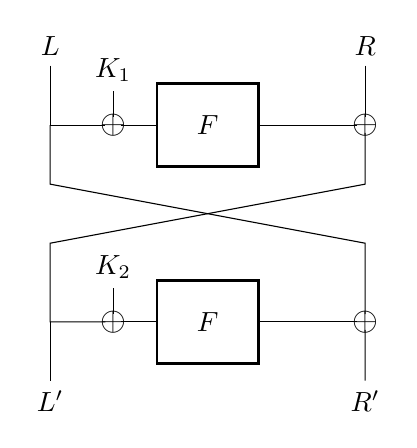
\begin{tikzpicture}[auto,transform shape]
    \tikzstyle{block} = [rectangle, draw, thick,
        text width=3em, text centered, minimum height=3em]
    \tikzstyle{line} = [draw, -]
    
    \node [block] (Et) {$F$};
    \coordinate [above of=Et, node distance=1cm] (top);
    \coordinate [left of=Et, node distance=2cm] (midleft);
    \node [left of=top, node distance=2cm] (m1) {$L$};
    \node [left of=Et, node distance=1.2cm, thick, scale=1.2] (xor1) {$\mathbf{\oplus}$};
    \node [above of=xor1, node distance=0.7cm] (4L1) {$K_{1}$};
    \coordinate [left of=xor1, node distance=1mm] (xor11);
    \path [line] (m1) -- (midleft) -- (xor11);
    \coordinate [above of=xor1, node distance=1mm] (xor12);
    \path [line] (4L1) -- (xor12);
    \coordinate [right of=xor1, node distance=1mm] (xor13);
    \path [line] (xor13) -- (Et);
    %
    \node [right of=top, node distance=2cm] (m2) {$R$};
    \node [right of=Et, node distance=2cm, thick, scale=1.2] (xor2) {$\mathbf{\oplus}$};
    \coordinate [left of=xor2, node distance=1mm] (xor21);
    \path [line] (Et) -- (xor21);
    \coordinate [above of=xor2, node distance=1mm] (xor22);
    \path [line] (m2) -- (xor22);
    %
    \coordinate [below of=midleft, node distance=.75cm] (botleft);
    \coordinate [below of=botleft, node distance=.75cm] (bumleft);
    \coordinate [right of=botleft, node distance=4cm] (botright);
    \coordinate [right of=bumleft, node distance=4cm] (bumright);
    \coordinate [below of=xor2, node distance=1mm] (xor23);
    \node [block, below of=Et, node distance=2.5cm] (Eb) {$F$};
    %
    \coordinate [left of=Eb, node distance=2cm] (bimleft);
    \node [left of=Eb, node distance=1.2cm, thick, scale=1.2] (xor3) {$\mathbf{\oplus}$};
    \coordinate [left  of=xor3, node distance=1mm] (xor31);
    \coordinate [above of=xor3, node distance=1mm] (xor32);
    \coordinate [right of=xor3, node distance=1mm] (xor33);
    \coordinate [below of=xor3, node distance=1mm] (xor34);
    \node [above of=xor3, node distance=0.7cm] (4L2) {$K_{2}$};
    %
    \path [line] (xor23) -- (botright) -- (bumleft) -- (bimleft) -- (xor31);
    \path [line] (4L2) -- (xor32);
    \path [line] (xor33) -- (Eb);
    %
    \node [right of=Eb, node distance=2cm, thick, scale=1.2] (xor4) {$\mathbf{\oplus}$};
    \coordinate [below of=xor4, node distance=1mm] (xor41);
    \coordinate [left of=xor4, node distance=1mm] (xor42);
    \coordinate [above of=xor4, node distance=1mm] (xor43);
    \path [line] (midleft) -- (botleft) -- (bumright) -- (xor43);
    \path [line] (Eb) -- (xor42);
    %
    \node [below of=m1, node distance=4.5cm] (c1) {$L'$};
    \node [right of=c1, node distance=4cm] (c2) {$R'$};
    \path [line] (bimleft) -- (c1);
    \path [line] (xor41) -- (c2);
    
    \end{tikzpicture}
    \caption{Fiestel Structure}
    \label{fig:fiestel}
\end{figure}
\newpage
\section{Sponge Construction}

Sponge construction is a flexible and innovative framework used in various cryptographic algorithms. It is designed to process input data of various length and produce an output of a desired size, making the algorithm highly adaptable for different cryptographic needs.

\subsection{Structure}
The sponge construction operates in two main stages:

\begin{itemize}
    \item \textbf{Absorbing Stage:} The input message is divided into fixed-size blocks, and each block is absorbed into the internal state of the sponge function. The state is updated iteratively using a permutation function.
    \item \textbf{Squeezing Stage:} Once the entire message is absorbed, the internal state is used to produce the output. This phase generates output blocks by applying the permutation function and extracting parts of the state.
\end{itemize}

The internal part of the sponge function is consist of two parts: a capacity part (providing security) and a bitrate part (determining the rate of data absorption and output). Basic structure of Sponge is shown in Figure \ref{fig:sponge}

\newpage
\subsection{Design Principles}

\begin{itemize}
    \item The ability to handle input and output of varying lengths makes sponge construction suitable for various cryptographic applications.
    
    \item The iterative process of absorption and squeezing allows for efficient processing of data, making it suitable for high-speed and resource-constrained environments.
\end{itemize}

\begin{figure}
    \centering
    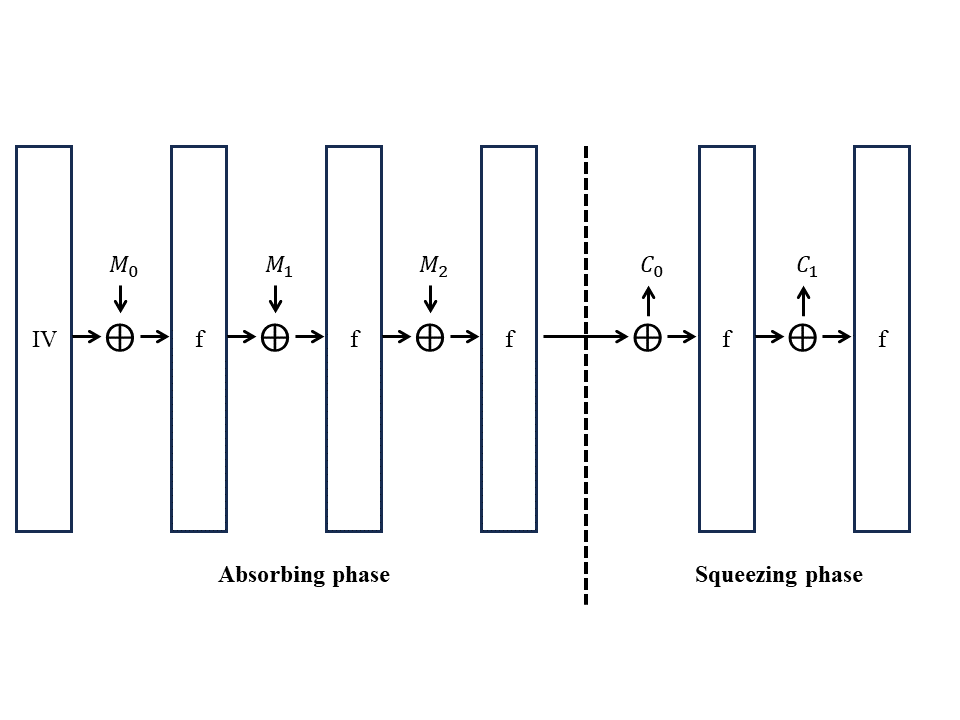
\includegraphics[width=0.9\linewidth]{fig/sponge.png}
    \caption{Sponge Constraction}
    \label{fig:sponge}
\end{figure}

\subsection{Example: ASCON}

ASCON \cite{dobraunig2014ascon} is a lightweight  cryptographic algorithm that employs sponge construction, designed specifically for applications in resource-limited environments such as the Internet of Things (IoT). ASCON provides both authenticated encryption and hashing functionalities.

\begin{itemize}
    \item \textbf{Initialization:} The internal state is initialized with a fixed initial value and the key, nonce, and other parameters are absorbed into the state.
    \item \textbf{Absorption:} The message blocks are absorbed into the state through a series of iterations involving a permutation function. 
    \item \textbf{Squeezing:} After the entire message is absorbed, the state is squeezed to produce the ciphertext and authentication tag. The squeezing phase involves applying the permutation function and extracting parts of the state to form the output.
\end{itemize}

\section{ARX (Addition-Rotation-XOR)}

ARX ciphers consist of  combination of three opetaions: addition modulo $2^n$, bitwise rotation, and bitwise XOR. 

\subsection{Structure}
An ARX-based ciphers typically involves a series of rounds, each consisting of the following operations:

\begin{itemize}
    \item \textbf{Addition:} Modular addition (usually modulo $2^n$) is used to combine key and data words, providing non-linearity.
    \item \textbf{Rotation:} Bitwise rotation shifts the bits of a word, ensuring that all bits influence the output and contributing to diffusion.
    \item \textbf{XOR:} It is used for combining intermediate results with round keys.
\end{itemize}


\subsection{Design Principles}


\begin{itemize}
    \item ARX operations are simple and efficient to implement in software, making them suitable for high-speed encryption.
    \item Bitwise rotation makes changes in the intermediate results distribute through the state, providing diffusion.
    \item Modular addition introduce non-linearity, making it difficult for attackers to predict intermediate states.
\end{itemize}

\newpage
\subsection{Example: Speck}
Speck \cite{beaulieu2015simon} is an ARX-based block cipher designed by the NSA for lightweight applications. It uses a simple structure that combines the ARX operations to provide security while maintaining performance in constrained environments. Speck comes in multiple variants like Speck32/64 and Speck128/256. Firs parameter is block size nad second parameter is key size.



\begin{figure}
    \centering
    
\includegraphics[width=0.9\linewidth]{fig/speck.png}
    \caption{ARX example Speck's round function}
    \label{fig:speck}
\end{figure}

\subsubsection{Encryption Process and Key Schedule}
The encryption process in Speck involves a sequence of ARX operations applied over multiple rounds. Example of ARX cipher Speck's round function shown in Figure \ref{fig:speck}


